\documentclass{beamer}
\usepackage[utf8]{inputenc}

\usetheme{Madrid}
\usecolortheme{default}
\usepackage{amsmath,amssymb,amsfonts,amsthm}
\usepackage{txfonts}
\usepackage{tkz-euclide}
\usepackage{listings}
\usepackage{adjustbox}
\usepackage{array}
\usepackage{tabularx}
\usepackage{gvv}
\usepackage{lmodern}
\usepackage{circuitikz}
\usepackage{tikz}
\usepackage{graphicx}
\usepackage{textcomp}
\usepackage{cancel}
\setbeamertemplate{page number in head/foot}[totalframenumber]

\usepackage{tcolorbox}
\tcbuselibrary{minted,breakable,xparse,skins}



\definecolor{bg}{gray}{0.95}
\DeclareTCBListing{mintedbox}{O{}m!O{}}{%
  breakable=true,
  listing engine=minted,
  listing only,
  minted language=#2,
  minted style=default,
  minted options={%
    linenos,
    gobble=0,
    breaklines=true,
    breakafter=,,
    fontsize=\small,
    numbersep=8pt,
    #1},
  boxsep=0pt,
  left skip=0pt,
  right skip=0pt,
  left=25pt,
  right=0pt,
  top=3pt,
  bottom=3pt,
  arc=5pt,
  leftrule=0pt,
  rightrule=0pt,
  bottomrule=2pt,
  toprule=2pt,
  colback=bg,
  colframe=orange!70,
  enhanced,
  overlay={%
    \begin{tcbclipinterior}
    \fill[orange!20!white] (frame.south west) rectangle ([xshift=20pt]frame.north west);
    \end{tcbclipinterior}},
  #3,
}
\lstset{
    language=C,
    basicstyle=\ttfamily\small,
    keywordstyle=\color{blue},
    stringstyle=\color{orange},
    commentstyle=\color{green!60!black},
    numbers=left,
    numberstyle=\tiny\color{gray},
    breaklines=true,
    showstringspaces=false,
}
%------------------------------------------------------------
%This block of code defines the information to appear in the
%Title page
\title %optional
{9.2.11}
\date{}
%\subtitle{A short story}

\author % (optional)
{Sai Krishna Bakki - EE25BTECH11049}

\begin{document}
\frame{\titlepage}
\begin{frame}{Question}
Find the area of the region bounded by the curve $y^2 = 9x$ and the lines $x = 2$ and $x = 4$ and the x-axis in the first quadrant.
\end{frame}
\begin{frame}{Theoretical Solution}
    The general equation of a conic section is given by $\vec{x}^\top\vec{V}\vec{x} + 2\vec{u}^\top\vec{x} + f = 0$, where $\vec{x} = \myvec{x \\ y}$.
The parameters of the conic are
\begin{align}
\vec{V} = \myvec{0 & 0 \\ 0 & 1}, \quad \vec{u} = \myvec{-9/2 \\ 0}, \quad f = 0
\end{align}

For the line x - 2 = 0, the parameters are
\begin{align}
\vec{h}_1 = \myvec{2 \\ 0}, \quad \vec{m}_1 = \myvec{0 \\ 1}
\end{align}
The parameter $\kappa$ for the points of intersection is found using the formula:
\begin{align}
\kappa = \frac{1}{\vec{m}^\top \vec{V} \vec{m}}\brak{-\vec{m}^\top(\vec{V}\vec{h}+\vec{u}) \pm \sqrt{\sbrak{\vec{m}^\top(\vec{V}\vec{h}+\vec{u})}^2 - g(\vec{h})(\vec{m}^\top \vec{V} \vec{m})}}
\end{align}
where $g(\vec{h}) = \vec{h}^\top \vec{V} \vec{h} + 2\vec{u}^\top \vec{h} + f$.
\end{frame}
\begin{frame}{Theoretical Solution}
Substituting the values into the formula for $\kappa$:
\begin{align}
\kappa &= \brak{-0 \pm \sqrt{0^2 - (-18)(1)}} = 3\sqrt{2},-3\sqrt{2}
\end{align}
yielding the points of intersection
\begin{align}
\vec{a}_0 =  \myvec{2 \\ 3\sqrt{2}},\vec{a}_1 =  \myvec{2 \\ -3\sqrt{2}}
\end{align}

For the line x - 4 = 0, the parameters are:
\begin{align}
\vec{h}_2 = \myvec{4 \\ 0}, \quad \vec{m}_2 = \myvec{0 \\ 1}
\end{align}

\begin{align}
\kappa &= \frac{1}{1}\brak{-0 \pm \sqrt{0^2 - (-36)(1)}} = 6,-6
\end{align}
yielding the points of intersection
\begin{align}
\vec{a}_2 = \myvec{4 \\ 6},\vec{a}_3 = \myvec{4 \\ -6}
\end{align}
\end{frame}
\begin{frame}{Theoretical Solution}
Thus, the area of the parabola in between the lines x = 2 and
x = 4 is given by
\begin{align}
A &= \int_{0}^{4} 3\sqrt{x} \, dx -\int_{0}^{2} 3\sqrt{x}\,dx  \\
&= 16 - 4\sqrt{2}
\end{align}
Thus, the area of the specified region is 16 - 4$\sqrt{2}$ square units.
\end{frame}
\begin{frame}[fragile]
\frametitle{C Code}
\begin{lstlisting}
#include <math.h>

/**
 * @brief Defines the parabola y = 3*sqrt(x) for the first quadrant.
 * * @param x The x-coordinate.
 * @return The corresponding y-coordinate.
 */
double parabola_func(double x) {
    return 3.0 * sqrt(x);
}

/**
 * @brief Calculates the definite integral of the parabola function 
 * using the trapezoidal rule.
 * * @param a The lower limit of integration.
 * @param b The upper limit of integration.
 \end{lstlisting}
 \end{frame}
\begin{frame}[fragile]
\frametitle{C Code}
\begin{lstlisting}
 * @param n The number of trapezoids (steps) to use for the approximation.
 * @return The calculated area under the curve in the first quadrant.
 */
double trapezoidal_area(double a, double b, int n) {
    double h = (b - a) / n;
    // Initialize sum with the first and last terms of the trapezoidal rule
    double sum = 0.5 * (parabola_func(a) + parabola_func(b));
    
    // Add the intermediate terms
    for (int i = 1; i < n; i++) {
        sum += parabola_func(a + i * h);
    }

    return h * sum;
}
 \end{lstlisting}
 \end{frame}
\begin{frame}[fragile]
\frametitle{Python Code Uses ctypes}
\begin{lstlisting}
# Program to plot the area under a parabola using a C backend for calculation.
# Based on code by GVV Sharma
# Python script by user, C integration by Gemini

import numpy as np
import matplotlib.pyplot as plt
import ctypes
import os
import sys

# --- Local Imports Setup ---
# Update this path to the location of your 'CoordGeo' scripts

try:
    from libs.line.funcs import *
    from libs.triangle.funcs import *
    from libs.conics.funcs import *
     \end{lstlisting}
 \end{frame}
\begin{frame}[fragile]
\frametitle{Python Code Uses ctypes}
\begin{lstlisting}
except ImportError:
    print(" ")
# --- End Local Imports Setup ---

# --- 1. Compile and Load the C Library ---

# Define file names
c_source = "area_lib.c"
lib_name = "area_lib.so"

# Compilation command (for Linux/macOS). For Windows, this would be different.


# Load the compiled shared library
try:
    area_lib = ctypes.CDLL(os.path.abspath(lib_name))
except OSError as e:
 \end{lstlisting}
 \end{frame}
\begin{frame}[fragile]
\frametitle{Python Code Uses ctypes}
\begin{lstlisting}
    print(f"Error loading shared library: {e}")
    sys.exit(1)


# --- 2. Define the C function signature for Python ---

# Get the function from the library
trapezoidal_area_c = area_lib.trapezoidal_area

# Specify the argument types (double, double, int)
trapezoidal_area_c.argtypes = [ctypes.c_double, ctypes.c_double, ctypes.c_int]
# Specify the return type (double)
trapezoidal_area_c.restype = ctypes.c_double


# --- 3. Define Parabola, Boundaries and Calculate Area ---
# The curve is y^2 = 9x
 \end{lstlisting}
 \end{frame}
\begin{frame}[fragile]
\frametitle{Python Code Uses ctypes}
\begin{lstlisting}
def parabola_x(y):
    """Returns the x-coordinate for a given y on the parabola y^2 = 9x."""
    return (y**2) / 9
# Boundaries
x_min = 2
x_max = 4
# Call the C function to get the area for the first quadrant
area_first_quadrant = trapezoidal_area_c(ctypes.c_double(x_min), ctypes.c_double(x_max), ctypes.c_int(1000))
# The total area is symmetric, so we double the result
total_area = 2 * area_first_quadrant
print(f"The calculated total area (from C function) is: {total_area}")
# --- 4. Find Intersection Points for Plotting ---
y1 = np.sqrt(9 * x_min)
y2 = np.sqrt(9 * x_max)
a2 = np.array([x_max, y2])
a1 = np.array([x_min, y1])
 \end{lstlisting}
 \end{frame}
\begin{frame}[fragile]
\frametitle{Python Code Uses ctypes}
\begin{lstlisting}
a0 = np.array([x_min, -y1])
a3 = np.array([x_max, -y2])
points = np.vstack((a0, a1, a2, a3)).T
point_labels = ['$\\mathbf{a}_0$', '$\\mathbf{a}_1$', '$\\mathbf{a}_2$', '$\\mathbf{a}_3$']
# --- 5. Set up the Plot ---
fig = plt.figure()
ax = fig.add_subplot(111)

# Generate data for plotting
y_curve = np.linspace(-7, 7, 400)
x_curve = parabola_x(y_curve)
x_fill = np.linspace(x_min, x_max, 100)
y_fill_pos = np.sqrt(9 * x_fill)
y_fill_neg = -np.sqrt(9 * x_fill)
# Plot the elements
ax.plot(x_curve, y_curve, 'r', label='Parabola')
ax.plot([a0[0], a1[0]], [a0[1], a1[1]], color='dodgerblue', label='Chord')
 \end{lstlisting}
 \end{frame}
\begin{frame}[fragile]
\frametitle{Python Code Uses ctypes}
\begin{lstlisting}
ax.plot([a3[0], a2[0]], [a3[1], a2[1]], color='darkorange', label='Chord')
ax.fill_between(x_fill, y_fill_pos, y_fill_neg, color='cyan', label=f'Area $\\approx$ {total_area:.4f}')
ax.scatter(points[0, :], points[1, :], s=30, color='dimgray')
for i, txt in enumerate(point_labels):
    ax.annotate(txt, (points[0, i], points[1, i]), textcoords="offset points", xytext=(5,5), ha='center')
# --- 6. Formatting and Display ---
ax.spines['left'].set_position('zero')
ax.spines['bottom'].set_position('zero')
ax.spines['right'].set_color('none')
ax.spines['top'].set_color('none')
ax.xaxis.set_ticks_position('bottom')
ax.yaxis.set_ticks_position('left')
plt.xlim(-1, 7)
plt.ylim(-7, 7)
ax.grid(True)
ax.legend(loc='upper left') plt.show()
 \end{lstlisting}
 \end{frame}
\begin{frame}[fragile]
\frametitle{Python Code}
\begin{lstlisting}
# Program to plot the area under a parabola
# Based on code by GVV Sharma
# Revised to match a specific plot style.

import numpy as np
import matplotlib.pyplot as plt

# --- Local Imports Setup ---
import sys
# Update this path to the location of your 'CoordGeo' scripts
sys.path.insert(0, '/sdcard/github/matgeo/codes/CoordGeo')

# Local imports from your custom geometry library
# Note: These specific functions are not used in this area calculation,
# but the structure is included for consistency with your other projects.
try:
    from libs.line.funcs import *
     \end{lstlisting}
 \end{frame}
\begin{frame}[fragile]
\frametitle{Python Code}
\begin{lstlisting}
    from libs.triangle.funcs import *
    from libs.conics.funcs import *
except ImportError:
    print("Generating Plot")
# --- End Local Imports Setup ---
# --- 1. Define the Parabola and Bounding Lines ---
# The curve is y^2 = 9x
def parabola_x(y):
    """Returns the x-coordinate for a given y on the parabola y^2 = 9x."""
    return (y**2) / 9
# Boundaries
x_min = 2
x_max = 4
# --- 2. Find Intersection Points ---
y1 = np.sqrt(9 * x_min)  # y-coordinate at x=2
y2 = np.sqrt(9 * x_max)  # y-coordinate at x=4
 \end{lstlisting}
 \end{frame}
\begin{frame}[fragile]
\frametitle{Python Code}
\begin{lstlisting}
# Points are labeled counter-clockwise from the top right
a2 = np.array([x_max, y2])
a1 = np.array([x_min, y1])
a0 = np.array([x_min, -y1])
a3 = np.array([x_max, -y2])

points = np.vstack((a0, a1, a2, a3)).T
point_labels = ['$\\mathbf{a}_0$', '$\\mathbf{a}_1$', '$\\mathbf{a}_2$', '$\\mathbf{a}_3$']

# --- 3. Set up the Plot ---
fig = plt.figure()
ax = fig.add_subplot(111)

# Generate y values for a smooth parabola curve
y_curve = np.linspace(-7, 7, 400)
x_curve = parabola_x(y_curve)
 \end{lstlisting}
 \end{frame}
\begin{frame}[fragile]
\frametitle{Python Code}
\begin{lstlisting}
# Generate x values for the shaded area
x_fill = np.linspace(x_min, x_max, 100)
y_fill_pos = np.sqrt(9 * x_fill)
y_fill_neg = -np.sqrt(9 * x_fill)

# --- 4. Plot the Elements ---

# Plot the parabola
ax.plot(x_curve, y_curve, 'r', label='Parabola')

# Plot the chords (vertical lines)
ax.plot([a0[0], a1[0]], [a0[1], a1[1]], color='dodgerblue', label='Chord')
ax.plot([a3[0], a2[0]], [a3[1], a2[1]], color='darkorange', label='Chord') # Second label is for legend entry

# Shade the area between the curves
ax.fill_between(x_fill, y_fill_pos, y_fill_neg, color='cyan', label='Area')
 \end{lstlisting}
 \end{frame}
\begin{frame}[fragile]
\frametitle{Python Code}
\begin{lstlisting}
# Plot and label the intersection points
ax.scatter(points[0, :], points[1, :], s=30, color='dimgray')
for i, txt in enumerate(point_labels):
    ax.annotate(txt, (points[0, i], points[1, i]), textcoords="offset points", xytext=(5,5), ha='center')
# --- 5. Formatting and Display ---
# Center the axes at (0,0)
ax.spines['left'].set_position('zero')
ax.spines['bottom'].set_position('zero')
ax.spines['right'].set_color('none')
ax.spines['top'].set_color('none')
ax.xaxis.set_ticks_position('bottom')
ax.yaxis.set_ticks_position('left')
# Set axis limits
plt.xlim(-1, 7)
plt.ylim(-7, 7)
ax.grid(True)
ax.legend(loc='upper left')
plt.show()

\end{lstlisting}
\end{frame}
\begin{frame}{Plot By C code and Python Code}
    \begin{figure}
    \centering
    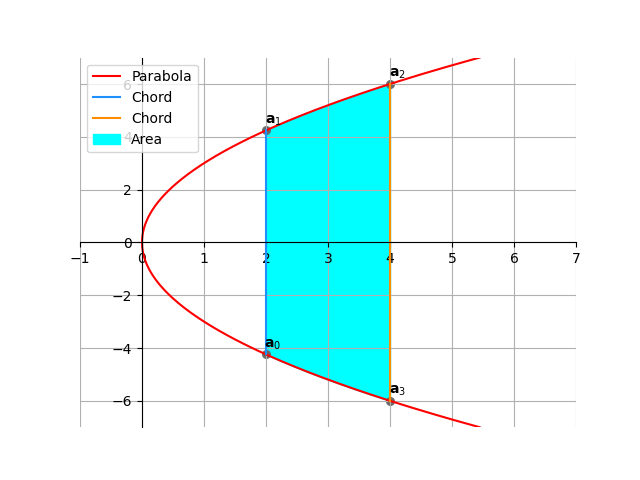
\includegraphics[width=0.7\columnwidth]{figs/Figure_1.png}
    \label{fig:placeholder}
    \caption{1}
\end{figure}
\end{frame}
\end{document}
